% AQUI VOCÊ CONTROLA QUAIS ELEMENTOS E CAPÍTULOS DEVEM SER EXIBIDOS, RECOMENDADO DESATIVAR AS ETAPAS QUE JÁ FORAM CONCLUÍDAS, ASSIM O ARQUIVO É COMPILADO MAIS RÁPIDO.
% os elementos pré-textuais devem ser modificados no main.tex
% o titulo, autor,instituição  e outros dados, devem ser informados no arquivo dadoDoTrabalho.tex

%%%%%%%%%%%%%%%%%%%%%%%%%%%%%%%%%%%%%%%%%%%%%%%%%%%%%%%%
% ELEMENTOS TEXTUAIS
%%%%%%%%%%%%%%%%%%%%%%%%%%%%%%%%%%%%%%%%%%%%%%%%%%%%%%%%
% ------------------------------------------------------
% introdução
% ------------------------------------------------------
\textual
	% exemplo de organização interna de um capítulo separando por mais de um arquivo

\chapter{Introdução}
\label{chap:introducao}
Esta é a primeira seção textual do trabalho onde se deve apresentar ideias, delimitando o assunto, bem como o objetivo geral e específico da pesquisa e outros. Elemento necessário para situar acerca da estrutura do trabalho.

Todo texto deve ser digitado em fonte times new roman ou arial, tamanho 12, inclusive a capa, com exceção das citações com mais de três linhas, notas de rodapé, paginação, dados internacionais de catalogação-na-publicação (ficha catalográfica), legendas e fontes das ilustrações e das tabelas, que devem ser em fonte times new roman ou arial, tamanho menor (10 ou 11). O texto deve ser justificado, exceto as referências, no final do trabalho, que devem ser alinhadas a esquerda.

Todos os autores citados devem ter a referência incluída em lista no final no trabalho.


 
 
\chapter{Texto Texto Texto}
\label{chap:intro}


 Texto \textit{text} texto texto texto texto texto texto texto texto texto texto texto texto texto texto texto texto texto texto texto texto texto texto texto texto texto texto texto texto texto texto texto texto texto texto texto, no \gls{MEC}.

 Segundo \citeonline{manualufpe2020}, o \gls{MEC}, texto texto texto texto texto texto texto texto texto texto texto texto texto texto texto texto texto texto texto texto texto texto texto texto texto texto texto texto texto texto texto texto texto texto texto texto .
 
 \begin{citacao}
 Texto \textit{text} texto texto texto texto texto texto texto texto texto texto texto texto texto texto texto texto texto texto texto texto texto texto texto texto texto texto texto texto texto texto texto texto texto texto texto texto texto texto texto texto texto \cite{manualufpe2020}.  
 \end{citacao}


 
 
\section{Texto Texto Texto}
\label{motivacao}

Texto texto texto texto texto texto texto texto texto texto texto texto texto texto texto texto texto texto texto texto texto texto texto texto texto texto texto texto texto texto texto texto texto texto texto texto, \textbf{exemplo} sigla \gls{SIBI}.

%você pode organizar melhor suas imagens se criar subpastas nos chapters
\begin{figure}[ht!]
\centering

\caption{\textmd{Texto Texto Texto Texto Texto Texto Texto Texto Texto Texto Texto Texto Texto Texto Texto Texto Texto Texto Texto Texto Texto Texto Texto Texto Texto Texto Texto Texto}}
\label{fig:figuraex}
\fcolorbox{gray}{white}{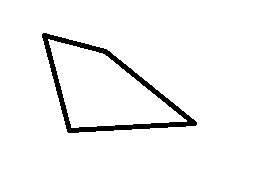
\includegraphics[width=0.5\textwidth]{ElementosTextuais/imagens/captitulo1/figuraex.png}}

\par\medskip\ABNTEXfontereduzida\selectfont\textbf{Fonte:} \citeauthor{manualufpe2020} (\citeyear{manualufpe2020}) \par\medskip
\end{figure}

Texto texto texto texto texto texto texto texto texto texto texto texto texto texto texto texto texto texto texto texto texto texto texto texto texto texto texto texto texto texto texto texto texto texto texto texto, conforme Figuras \ref{fig:figuraex} e Figuras \ref{fig:figuraex2}, continua no Capítulo %\ref{chap:outrocapitulo}.


\begin{figure}[ht!]
\centering

\caption{\textmd{Texto Texto Texto Texto Texto Texto Texto}}
\label{fig:figuraex2}
\fcolorbox{gray}{white}{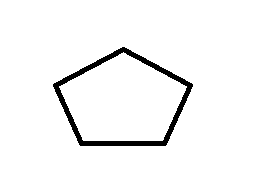
\includegraphics[width=0.80\textwidth]{ElementosTextuais/imagens/captitulo1/figuraex2.png}}

\par\medskip\ABNTEXfontereduzida\selectfont\textbf{Fonte:} \citeauthor{manualufpe2020} (\citeyear{manualufpe2020}) \par\medskip
\end{figure}

Texto texto texto texto texto texto texto texto texto texto texto texto texto texto texto texto texto texto texto texto texto texto texto texto texto texto texto \gls{UFPE}.

%\input{ElementosTextuais/Introducao/Capitulos/problemahipotese.tex}
\section{Texto Texto Texto}
\label{objetivos}
Texto texto texto texto texto texto texto texto texto texto texto texto texto texto texto texto texto texto texto texto texto texto texto texto texto texto texto texto texto texto texto texto texto texto texto texto.

Texto texto texto texto texto texto texto texto texto texto texto texto texto texto texto texto texto texto texto texto texto texto texto texto texto texto texto texto texto texto texto texto texto texto texto texto.

\subsection{Texto Texto Texto}
\label{sub:exemplonivel3}

Texto texto texto texto texto texto texto texto texto texto texto texto texto texto texto texto texto texto texto texto texto texto texto texto texto texto texto texto texto texto texto texto texto texto texto texto.

\subsubsection{Texto texto texto texto}
\label{subsub:exemplonivel4}

Texto texto texto texto texto texto texto texto texto texto texto texto texto texto texto texto texto texto texto texto texto texto texto texto texto texto texto texto texto texto texto texto texto texto texto texto.
%\input{ElementosTextuais/Introducao/Capitulos/organizacao.tex}
	\chapter{Texto Texto Texto}
\label{chap:outrocapitulo}

Texto texto texto texto ''texto'' texto texto texto texto texto texto texto texto texto texto texto texto texto texto texto texto texto texto texto texto texto texto texto texto texto texto texto texto texto texto texto, confome Tabela \ref{tbl:tabelaex} e a Tabela \ref{tbl:tabelaex2}.

%exemplo de inputs, ideal para organização e troca de posicionamento futuro é ter um elemento por arquivo

%usar um gerador é uma opção https://www.tablesgenerator.com/
% observação, segundo a biblioteca tableas não podem ter nenhuma linha vertical

\begin{table}[ht]
\caption{Texto Texto Texto}
\label{tbl:tabelaex}
\centering
\rowcolors{1}{}{lightgray}
\begin{tabular}{p{6cm}p{9cm}}
\hline
\multicolumn{1}{c}{\textbf{Coluna A}} & \multicolumn{1}{c}{\textbf{Coluna B}}  \\
\hline     
\textbf{coluna1} & Texto Texto Texto Texto Texto Texto Texto Texto Texto Texto Texto Texto.
\\ 

coluna2 & Texto Texto Texto Texto Texto Texto Texto Texto Texto Texto Texto Texto.              
\\ 

coluna3 & Texto \textit{Texto} Texto Texto Texto Texto Texto Texto Texto Texto Texto Texto.     
\\ \hline

\end{tabular}

  \par\medskip\ABNTEXfontereduzida\selectfont\textbf{Fonte:} Elaborada pelo autor (2020) \par\medskip
\end{table}



%usar um gerador é uma opção https://www.tablesgenerator.com/
% observação, segundo a biblioteca tableas não podem ter nenhuma linha vertical

\begin{table}[ht]
\caption{Texto Texto Texto}
\label{tbl:tabelaex2}
\centering
\rowcolors{1}{}{lightgray}
\begin{tabular}{p{6cm}p{9cm}}
\hline
\multicolumn{1}{c}{\textbf{Coluna A}} & \multicolumn{1}{c}{\textbf{Coluna B}}  \\
\hline 
coluna1 & Texto Texto Texto Texto Texto Texto ''Texto'' Texto Texto Texto Texto Texto.
\\ 

coluna2 & Texto Texto Texto Texto Texto Texto Texto Texto Texto Texto Texto Texto.              
\\

coluna3 & Texto \textit{Texto} Texto Texto Texto Texto Texto Texto Texto Texto Texto Texto.     
\\ \hline

\end{tabular}

  \par\medskip\ABNTEXfontereduzida\selectfont\textbf{Fonte:} \citeauthor{manualufpe2020} (\citeyear{manualufpe2020}) \par\medskip
\end{table}


\section{Texto Texto}
\label{sec:section}

Texto texto texto texto ''texto'' texto texto texto texto texto texto texto texto texto texto texto texto texto texto texto texto texto texto texto texto texto texto texto texto texto texto texto texto texto texto texto \cite{gil2002elaborar}.


\section{Texto Texto}
\label{sec:outrasection}

Texto texto texto texto ''texto'' texto texto texto texto texto texto texto texto texto texto texto texto texto texto texto texto texto texto texto texto texto texto texto texto texto texto texto texto texto texto texto

\subsection{Texto Texto Texto}
\label{sub:outrasubsectiona}

Texto texto texto texto ''texto'' texto texto texto texto texto texto texto texto texto texto texto texto texto texto texto texto texto texto texto texto texto texto texto texto texto texto texto texto texto texto texto


\subsubsection{Texto Texto Texto Texto}
\label{subsub:outrasubsubsection}

Texto texto texto texto ''texto'' texto texto texto texto texto texto texto texto texto texto texto texto texto texto texto texto texto texto texto texto texto texto texto texto texto texto texto texto texto texto texto

\subsubsection{Texto Texto Texto Texto}
\label{subsub:outrasubsubsection2a}

Texto texto texto texto ''texto'' texto texto texto texto texto texto texto texto texto texto texto texto texto texto texto texto texto texto texto texto texto texto texto texto texto texto texto texto texto texto texto

%a organização fica a seu critério se preferir utilize inputs para cada seção, subseção etc...
%apenas um exemplo de subseção em arquivo para ser incluido
\subsection{Texto Texto Texto}
%\label{sub:outrasubsection2}

Texto texto texto texto ''texto'' texto texto texto texto texto texto texto texto texto texto texto texto texto texto texto texto texto texto texto texto texto texto texto texto texto texto texto texto texto texto texto


\subsubsection{Texto Texto Texto Texto}
%\label{subsub:outrasubsubsection2}

Texto texto texto texto ''texto'' texto texto texto texto texto texto texto texto texto texto texto texto texto texto texto texto texto texto texto texto texto texto texto texto texto texto texto texto texto texto texto

%apenas um exemplo de subseção em arquivo para ser incluido

\section{Texto Texto}
\label{sec:section3}

Texto texto texto texto ''texto'' texto texto texto texto texto texto texto texto texto texto texto texto texto texto texto texto texto texto texto texto texto texto texto texto texto texto texto texto texto texto texto
	\chapter{Texto Texto Texto}
%não se esqueça de definir uma label única para utilizar no comando \ref
%\label{chap:metodologia}

Texto texto texto texto texto texto texto texto texto texto texto texto texto texto texto texto texto texto texto texto texto texto texto texto texto texto texto texto texto texto texto texto texto texto texto texto.

%exemplos de parágrafos com footnote
Texto texto texto texto texto texto texto texto texto texto texto texto texto texto texto texto texto texto texto texto texto texto texto texto texto texto texto texto texto texto texto texto texto texto texto texto \textit{Footnote} \footnote{Segundo \citeonline{manualufpe2020}, Exemplo de nota de rodapé.}.

\section{Texto Texto}
%\label{sec:algumlabel}

Texto texto texto texto texto texto texto texto texto texto texto texto texto texto texto texto texto texto texto texto texto texto texto texto texto texto texto texto texto texto texto texto texto texto texto texto.

Texto texto texto texto texto texto texto texto texto texto texto texto texto texto texto texto texto texto texto texto texto texto texto texto texto texto texto texto texto texto texto texto texto texto texto texto \textit{Footnote} \footnote{Segundo \citeonline{manualufpe2020}, Exemplo de nota de rodapé 2.}.

%exemplo de código fonte, as configurações estão no arquivo packages.tex
\lstinputlisting[language=PHP, 
caption=Texto texto texto texto
,label=lst:exemplocodigo1]{ElementosTextuais/antigo/trechos_codigo/funcoescatdinamicas.m}

\hspace{4cm}
\hfill
\begin{minipage}[t]{.65\textwidth}
\ABNTEXfontereduzida\selectfont\textbf{Fonte:} Elaborado pelo autor (2020) 
\end{minipage}


Texto texto texto texto texto texto texto texto texto texto texto texto texto texto texto texto texto texto texto texto texto texto texto texto texto texto texto texto texto texto texto texto texto texto texto texto, referente ao Código Fonte \ref{lst:exemplocodigo1} função \texttt{nome\_funcao}.

\subsection{Texto Texto Texto}
\label{subsec:algumlabel}

Texto texto texto texto texto texto texto texto texto texto texto texto texto texto texto texto texto texto texto texto texto texto texto texto texto texto texto texto texto texto texto texto texto texto texto texto.

\section{Texto Texto}
\label{sec:algumlabel2}
%exemplo de quadro
Texto texto texto texto texto texto texto texto texto texto texto texto texto texto texto texto texto texto texto texto texto texto texto texto texto texto texto texto texto texto texto texto texto texto texto texto, ver Quadro \ref{quad:exemplo_de_quadro}.

%a diferença do quadro pra tabela é que o quadro tem linhas verticais
\begin{quadro}
\caption{Texto texto texto texto texto}
\label{quad:exemplo_de_quadro}
\centering
\begin{tabular}{|lllll|}
\cline{1-5}
A& B &  C& D &E  \\ \cline{1-5}
\multirow{3}{*}{1}  & 2 &  3& 4& 5 \\
 &  2 &  3& 4& 5  \\
 &  2 &  3& 4& 5 \\
 \cline{1-5}
\end{tabular}
  \par\medskip\ABNTEXfontereduzida\selectfont\textbf{Fonte:} Elaborada pelo autor (2020) \par\medskip
\end{quadro}


\subsection{Texto Texto Texto}
\label{subsec:algumlabel2}
Texto texto texto texto texto texto texto texto texto texto texto texto texto texto texto texto texto texto texto texto texto texto texto texto texto texto texto texto texto texto texto texto texto texto texto texto.

\subsection{Texto Texto Texto}
\label{subsec:algumlabel3}

Texto texto texto texto texto texto texto texto texto texto texto texto texto texto texto texto texto texto texto texto texto texto texto texto texto texto texto texto texto texto texto texto texto texto texto texto.

	\chapter{Texto Texto Texto}
%\label{chap:capitulo1}

Texto texto texto texto texto texto texto texto texto texto texto texto texto texto texto texto texto texto texto texto texto texto texto texto texto texto texto texto texto texto texto texto texto texto texto texto.


\lstinputlisting[language=Java, 
caption=Texto texto texto texto
,label=lst:exemplocodigo2]{ElementosTextuais/antigo/trechos_codigo/java.m}
\hfill
\begin{minipage}[t]{.65\textwidth}
\ABNTEXfontereduzida\selectfont\textbf{Fonte:} \citeauthor{universidadejava2020}  (\citeyear{universidadejava2020}) 
\end{minipage}




\section{Texto Texto Texto}
%\label{sec:label}
Texto texto texto texto texto texto texto texto texto texto texto texto texto texto texto texto texto texto texto texto texto texto texto texto texto texto texto texto texto texto texto texto texto texto texto texto, ver Capítulo %\ref{chap:metodologia}, Seção \ref{sec:algumlabel}.

Texto texto texto texto texto texto texto texto texto texto texto texto texto texto texto texto texto texto texto texto texto texto texto texto texto texto texto texto texto texto texto texto texto texto texto texto (Código Fonte %\ref{lst:exemplocodigo2}).


\section{Texto Texto}
%\label{sec:outralabel}

Texto texto texto texto texto texto texto texto texto texto texto texto texto texto texto texto texto texto texto texto texto texto texto texto texto texto texto texto texto texto texto texto texto texto texto texto.


\bookmarksetup{startatroot}% 
% ------------------------------------------------------
% desenvolvimento
% ------------------------------------------------------

% ------------------------------------------------------
% conclusão
% ------------------------------------------------------


%%%%%%%%%%%%%%%%%%%%%%%%%%%%%%%%%%%%%%%%%%%%%%%%%%%%%%%%
% ELEMENTOS PÓS-TEXTUAIS
%%%%%%%%%%%%%%%%%%%%%%%%%%%%%%%%%%%%%%%%%%%%%%%%%%%%%%%%
\postextual

% ----------------------------------------------------------
% Referências bibliográficas
% ----------------------------------------------------------
%\bibliographystyle{abntexalfenglish} %caso seja em inglês, retire o comentário desta linha
% \renewcommand{\bibname}{REFER\^ENCIAS}
%\renewcommand{\bibname}{Bibliography}
% \addbibresource{mendeley.bib}
\bibliography{referencias}

% ------------------------------------------------------
% ademais
% ------------------------------------------------------
	

% ----------------------
% força para que não exiba subtítulos em apêndices no sumário
% -----------------------

\begin{apendicesenv}
\addtocontents{toc}{\protect\setcounter{tocdepth}{1}}
\makeatletter
\addtocontents{toc}{%
  \begingroup
  \let\protect\l@chapter\protect\l@section
  \let\protect\l@section\protect\l@subsection
}
\makeatother

% Imprime uma página indicando o início dos apêndices
% \partapendices

%coloca o identificador do anexo/apendice somente na primeira página
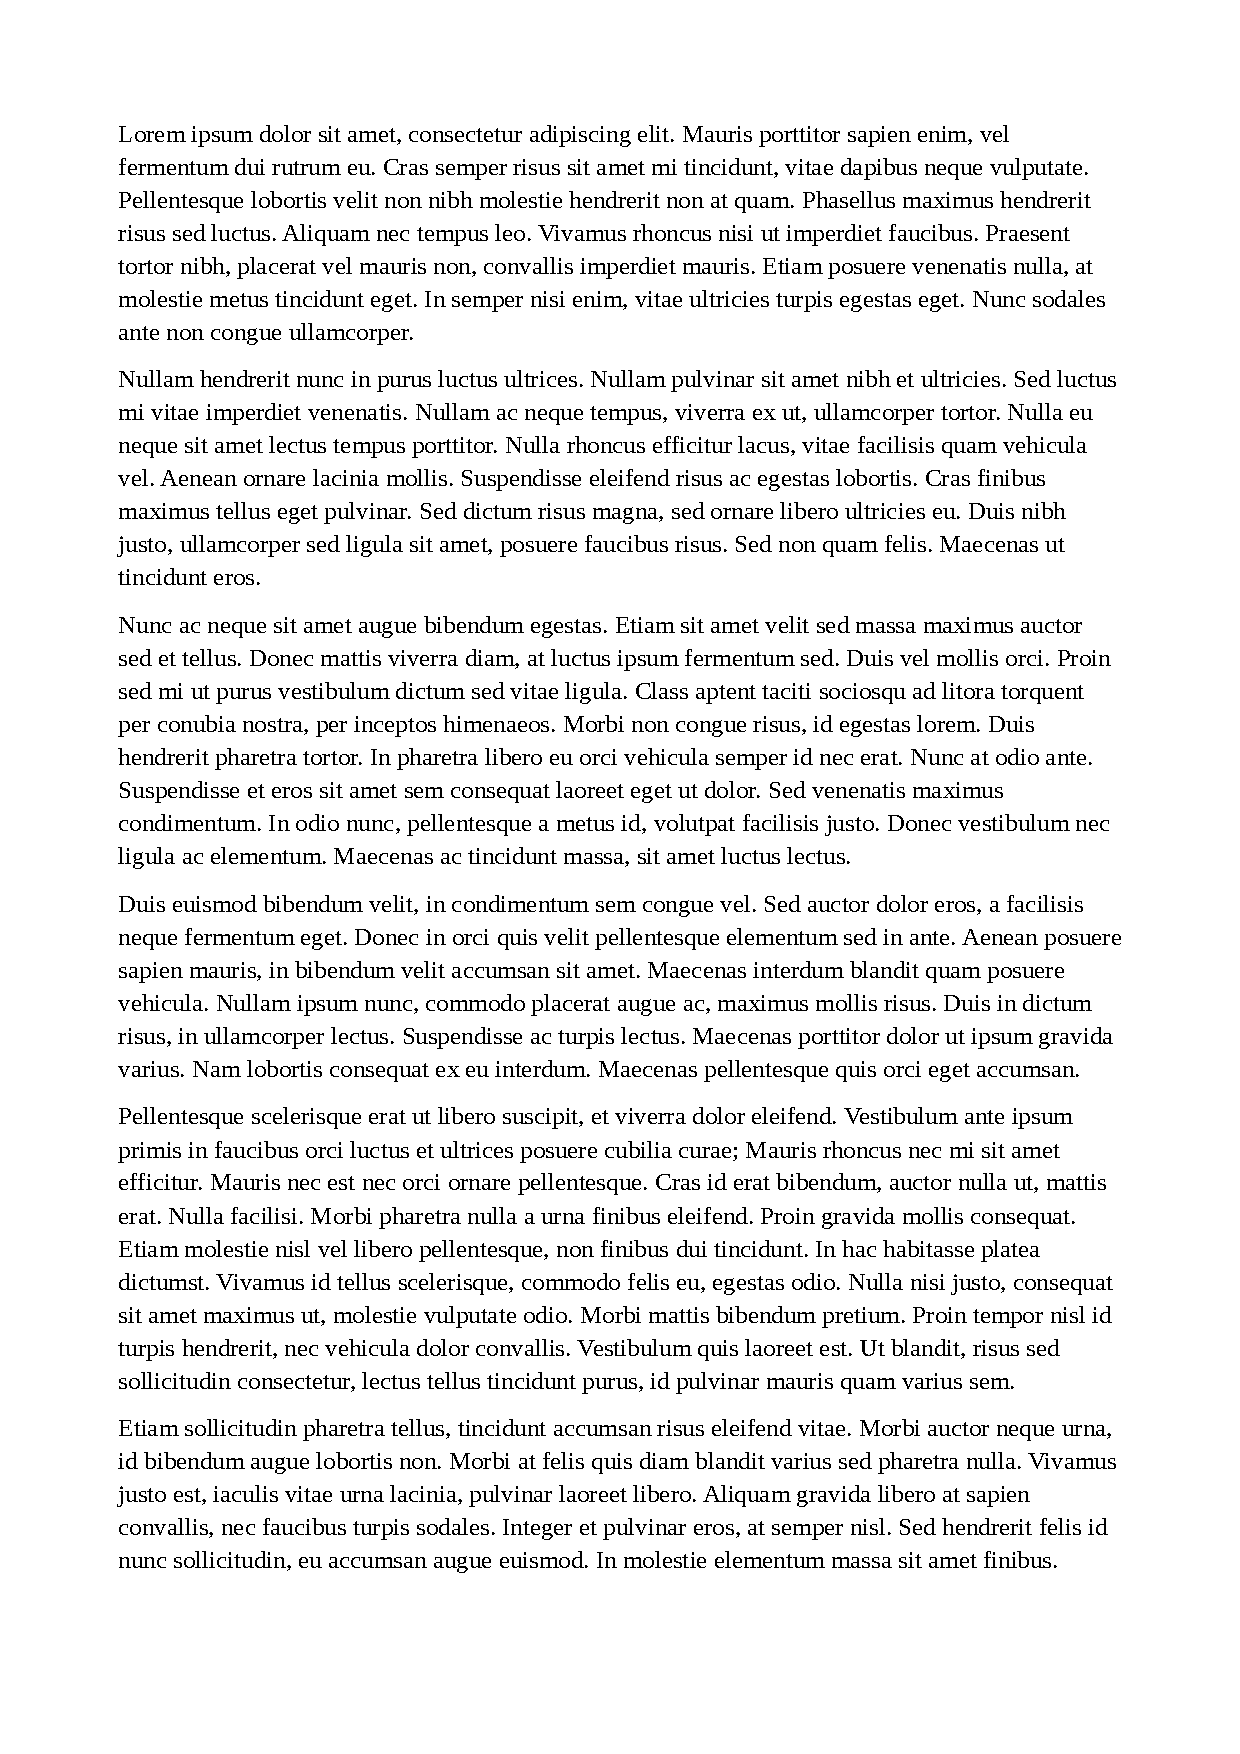
\includepdf[pages={1},scale=0.8,pagecommand=\chapter{Texto Texto Texto Texto}\label{apen:apendiceA}]{appendix/apendiceA}
\includepdf[pages={2-},scale=0.80,pagecommand={}]{appendix/apendiceA}

%coloca o identificador do anexo/apendice somente na primeira página
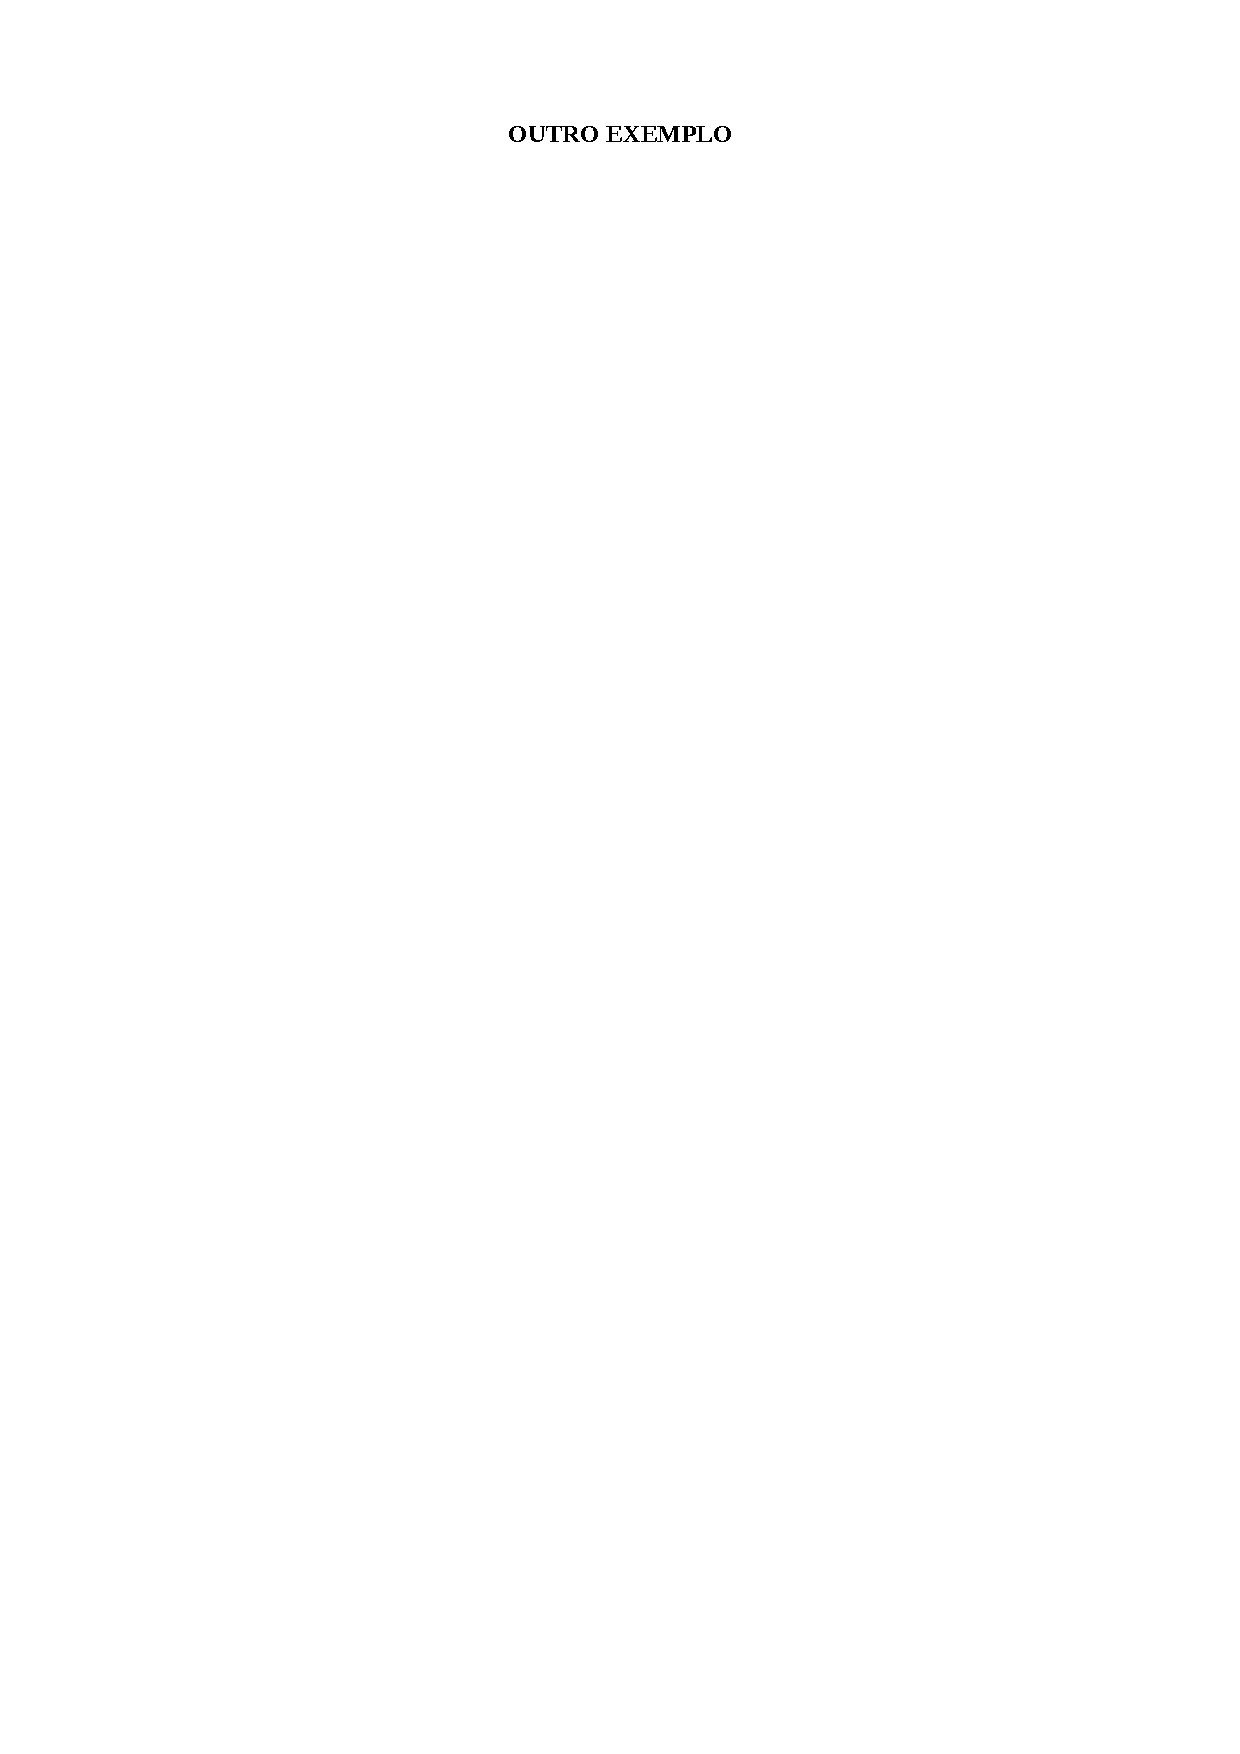
\includepdf[pages={1},scale=0.80,pagecommand=\chapter{Texto Texto Texto}\label{apen:apendiceB}]{ElementosPosTextuais/Apendice/apendiceB}


%coloca o identificador do anexo/apendice somente na primeira página
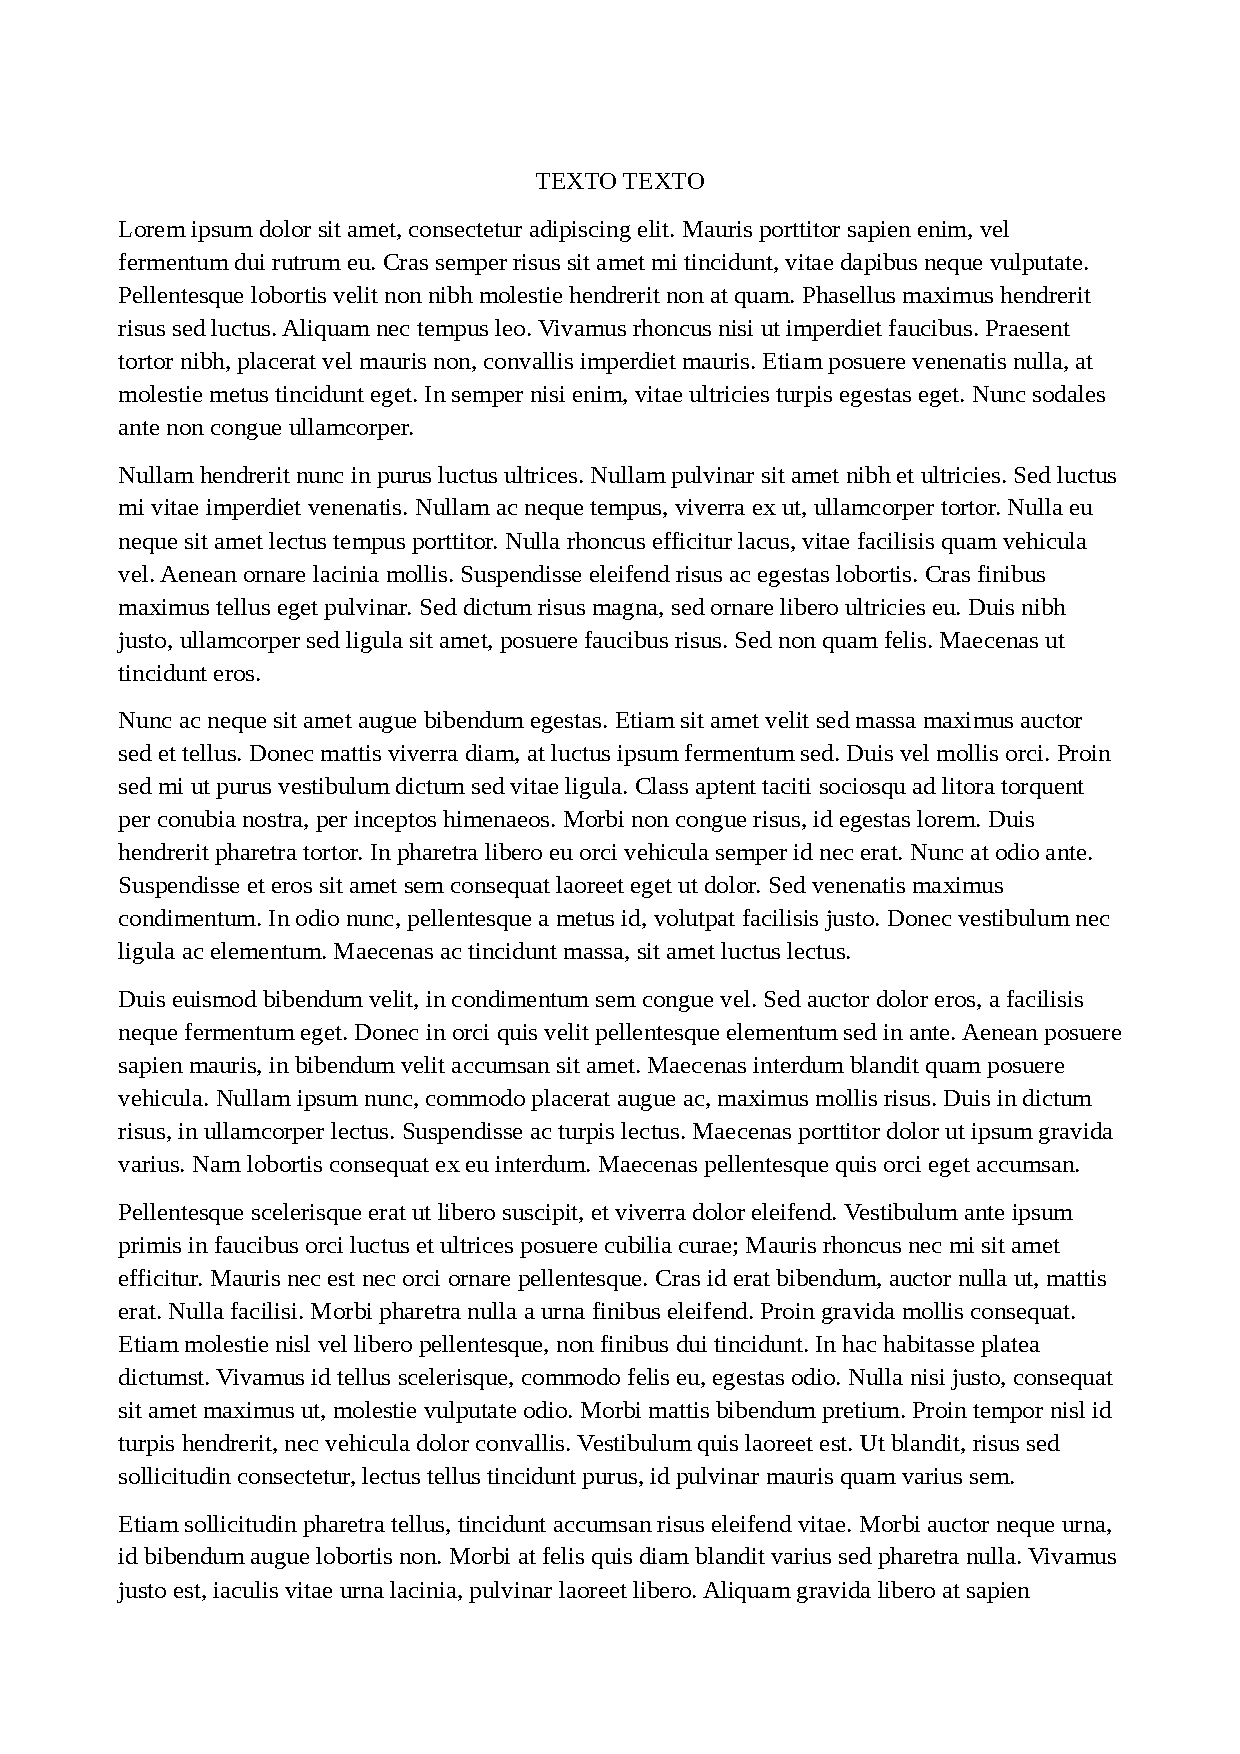
\includepdf[pages={1},scale=0.80,pagecommand=\chapter{Texto Texto}\label{apen:apendiceC}]{appendix/apendiceC}
\includepdf[pages={2},scale=0.80,pagecommand={}]{appendix/apendiceC}


\addtocontents{toc}{\endgroup}
\end{apendicesenv}



 % apendice
	
% ----------------------
% força para que não exiba subtítulos em apêndices no sumário
% -----------------------

\begin{anexosenv}
\addtocontents{toc}{\protect\setcounter{tocdepth}{1}}
\makeatletter
\addtocontents{toc}{%
  \begingroup
  \let\protect\l@chapter\protect\l@section
  \let\protect\l@section\protect\l@subsection
}
\makeatother
% Imprime uma página indicando o início dos apêndices
% \partapendices

%coloca o identificador do anexo/apendice somente na primeira página
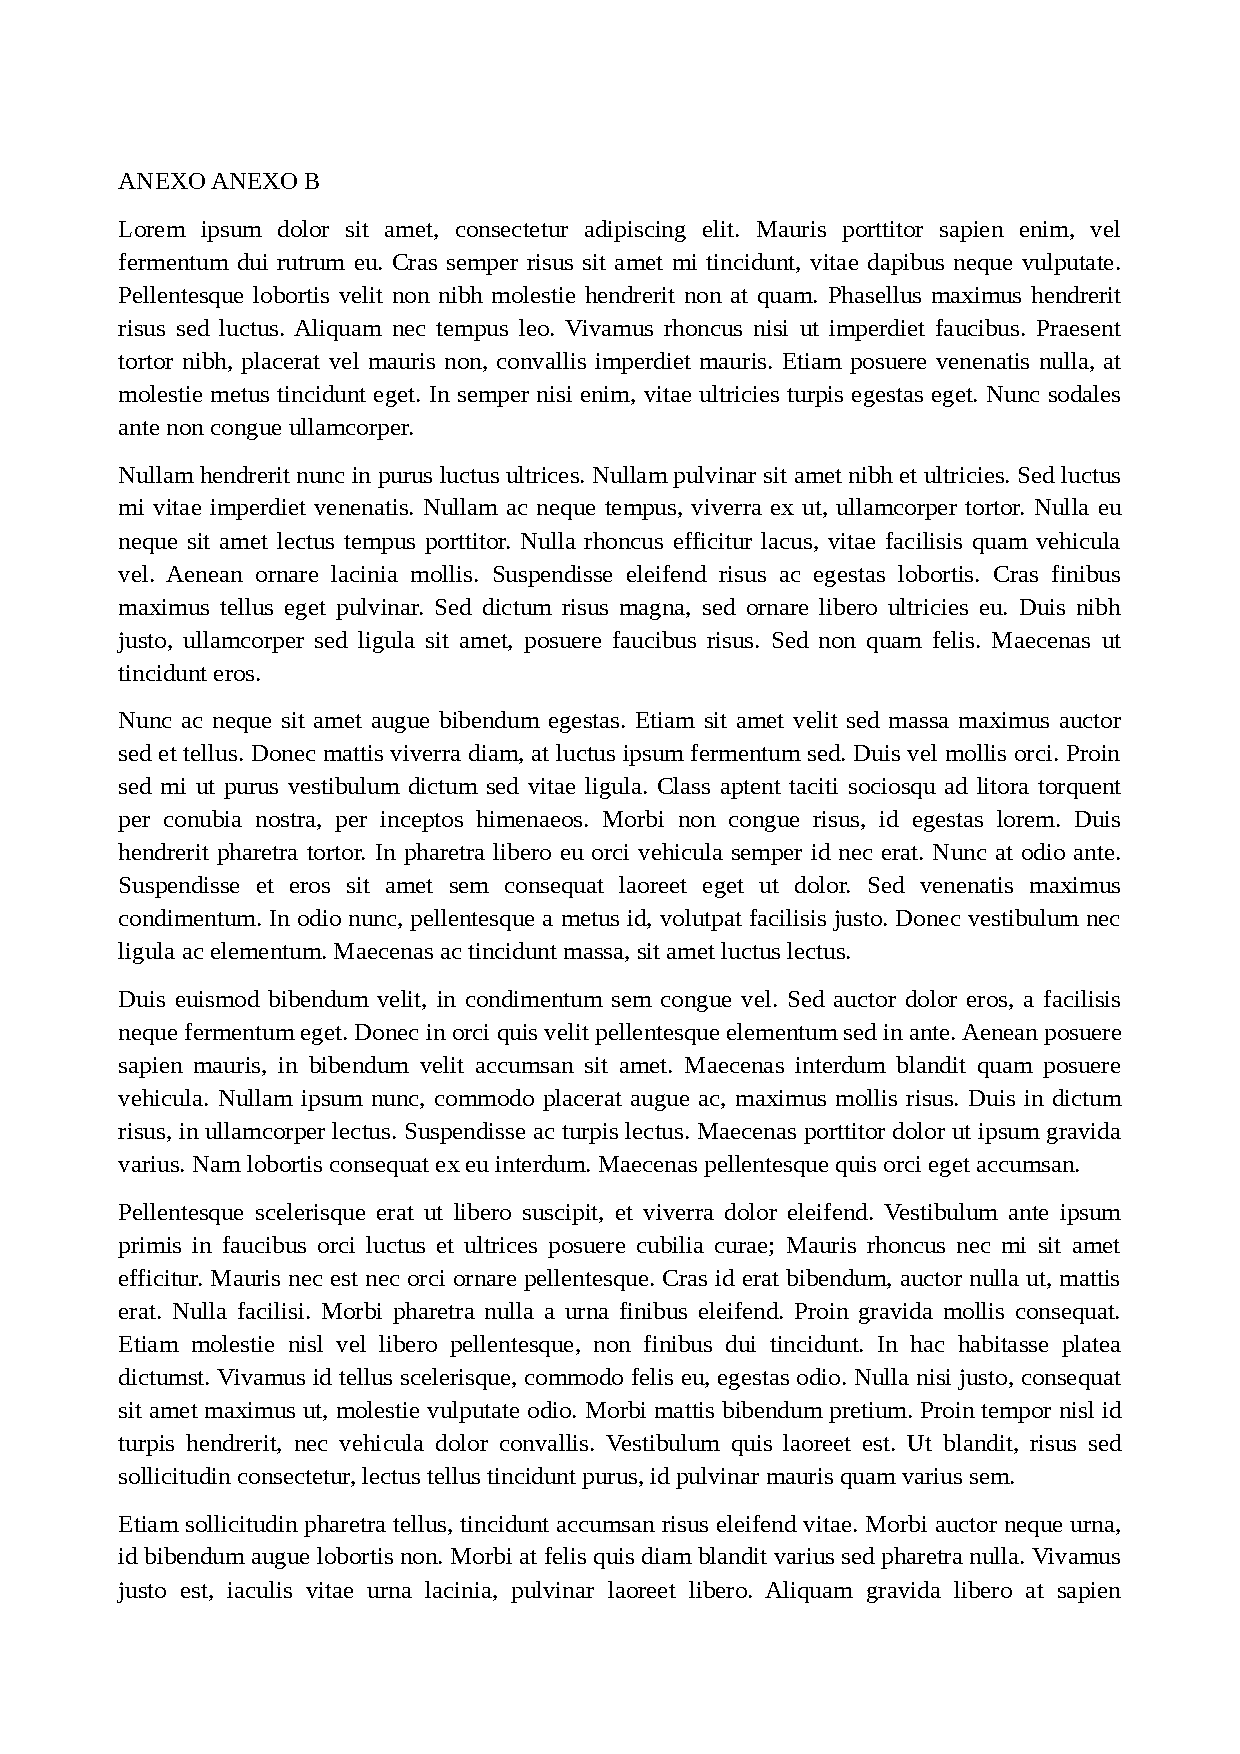
\includepdf[pages={1},scale=0.8,pagecommand=\chapter{Texto Texto Texto Texto}\label{anex:anexob}]{anexos/anexoB}
\includepdf[pages={2-},scale=0.80,pagecommand={}]{anexos/anexoB}

%coloca o identificador do anexo/apendice somente na primeira página
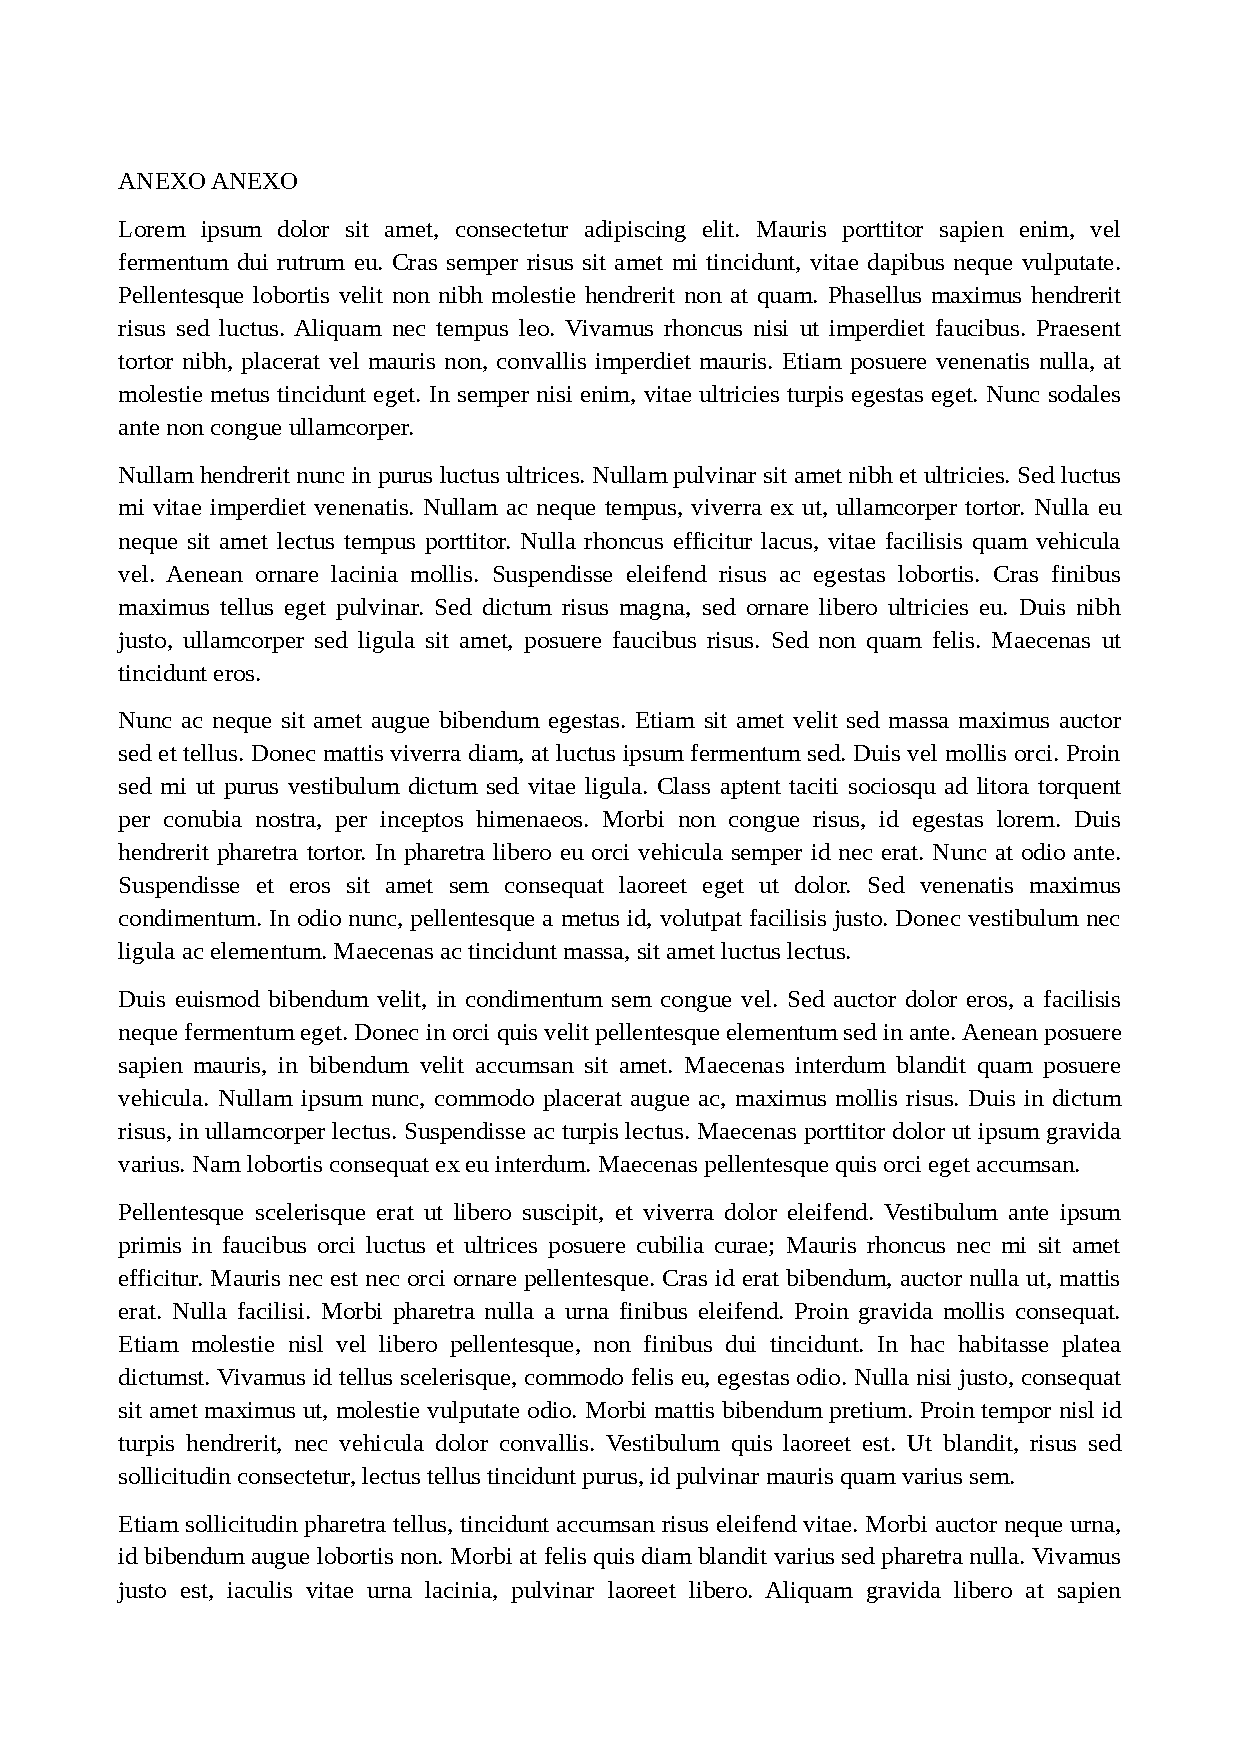
\includepdf[pages={1},scale=0.8,pagecommand=\chapter{Texto Texto Texto Texto}\label{anex:anexoa}]{anexos/anexoA}
\includepdf[pages={2-},scale=0.80,pagecommand={}]{anexos/anexoA}

\addtocontents{toc}{\endgroup}
\end{anexosenv}



 % anexos
%	
\newglossaryentry{naive-bayes}
{
  name=\textit{Na{\"i}ve Bayes},
  description={},
  plural=\textit{Na{\"i}ve Bayes}
}

\newglossaryentry{hoeffding-tree}
{
  name=\textit{Hoeffding Tree},
  description={},
  plural=\textit{Hoeffding Trees}
}












 % glossario

\printindex